\documentclass{article}
\usepackage{template}

\usepackage{chngcntr} % Reset counter within sections
\usepackage{circuitikz}

\counterwithin*{equation}{section}
\counterwithin*{equation}{subsection}

\pagestyle{fancy}
\setlength\headheight{24pt}

\lhead{\className}
\rhead{\leftmark}
\cfoot{\thepage}

\newcommand{\uniTitle}{Queensland University of Technology}
\newcommand{\className}{Foundations of Electrical Engineering}
\newcommand{\classTime}{Semester 2, 2021}
\newcommand{\classInstructorName}{Dr Jasmin Martin}
\newcommand{\authorName}{Tarang Janawalkar}
\newcommand{\authorStudentNumber}{n11032201}
\newcommand{\classCode}{EGB120}

\usepackage[
    type={CC},
    modifier={by-nc-sa},
    version={4.0},
    imagewidth={5em},
]{doclicense}

\date{}

\begin{document}
\begin{titlepage}
    \vspace*{\fill}
	\begin{center}
        \LARGE
        \textbf{\className}
        \texorpdfstring{\\}{ }
        \uniTitle
        \texorpdfstring{\\}{ }
        \texorpdfstring{\vspace{0.3in}}{ }
        \normalsize\textit{\classInstructorName}
        \texorpdfstring{\\}{ }
        \classTime
    \end{center}
    \begin{center}
        \textbf{\authorName}
    \end{center}
    \vspace*{\fill}
    \doclicenseThis
    \thispagestyle{empty}
\end{titlepage}
\newpage

\tableofcontents
\newpage

\section{Electrical Circuits}
\subsection{Fundamental Quantities}
\begingroup
\renewcommand{\arraystretch}{1.5}
\begin{table}[H]
    \centering
    \begin{tabular}{c | >{\centering}p{0.5\textwidth} | c c}
        \toprule
        \textbf{Name} & \textbf{Definition} & \textbf{Symbol} & \textbf{Unit} \\
        \midrule
        Charge & Electric charge is a fundamental property of matter that governs how particles are affected by an electromagnetic field.
        & $q$ & Coulomb (\unit{\coulomb}) \\
        \hline
        Current & $i=\dv{q}{t}\iff\SI{1}{\ampere}=\SI{1}{\coulomb\per\s}$
        & $i$ & Ampere (\unit{\ampere}) \\
        \hline
        Voltage & $v=\dv{w}{q}\iff\SI{1}{\volt}=\SI{1}{\joule\per\coulomb}$
        & $v$ & Volt (\unit{\volt}) \\
        \hline
        Power & $p=\dv{w}{t}\iff\SI{1}{\watt}=\SI{1}{\joule\per\s}$
        & $p$ & Watt (\unit{\watt}) \\
        \bottomrule
    \end{tabular}
\end{table}
\endgroup
\begin{description}
    \item[Charge in an electron.] $q=\SI{1.6022e-19}{\coulomb}$.
    \item[Electric Power.] $p=\dv{w}{t}=vi$. 
\end{description}
\subsection{Passive Sign Convention}
\begin{figure}[H]
    \centering
    \begin{minipage}[H]{0.48\textwidth}
        \textbf{Passive component}
        \centering
        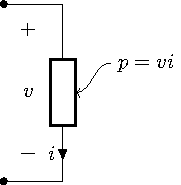
\includegraphics[height = 4cm, keepaspectratio = true]{passive_component}
        \caption{Energy dissipated.}
    \end{minipage}\hfill
    \begin{minipage}[H]{0.48\textwidth}
        \textbf{Active component}
        \centering
        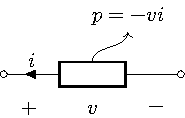
\includegraphics[height = 4cm, keepaspectratio = true]{active_component}
        \caption{Energy produced.}
    \end{minipage}
\end{figure}
\begin{theorem}[Power Balance]
    \begin{equation*}
        p_{\mathrm{net}} = 0
    \end{equation*}
\end{theorem}
\begin{theorem}[Energy]
    \begin{equation*}
        w\left( \tau \right) = \int_0^\tau p\left( t \right) \dd{t}
    \end{equation*}
\end{theorem}
\subsection{Circuits and Sources}
\begin{definition}[Circuits]
    A circuit is a mathematical model that approximates a real system. It is built from ideal circuit elements connected by ideal wires. 
\end{definition}
\begin{definition}[Voltage Source]
    Produces or dissipates power at a specified voltage with whatever current is required. 
\end{definition}
\begin{figure}[H]
    \centering
    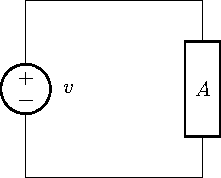
\includegraphics{voltage_source}
    \caption{Voltage Source -- $v$ is specified, $i$ varies depending on circuit element $A$.}
\end{figure}
\begin{definition}[Current Source]
    Produces or dissipates power at a specified current with whatever voltage is required. 
\end{definition}
\begin{figure}[H]
    \centering
    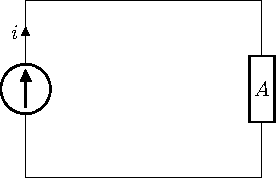
\includegraphics{current_source}
    \caption{Current Source -- $i$ is specified, $v$ varies depending on circuit element $A$.}
\end{figure}
% \subsection{Ground}
% \begin{description}
%     \item[Definition.] The zero volt point is referred to as the circuit ground.
%     \item[Symbol.] \tikz\draw (0, 0) node[sground] {};
% \end{description}
% \subsection{Earth}
% \begin{description}
%     \item[Definition.] An earthed ground is literally a connection to the earth.
%     \item[Symbol.] \tikz\draw (0, 0) node[ground] {};
% \end{description}
\subsection{Connected Sources}
\begin{figure}[H]
    \centering
    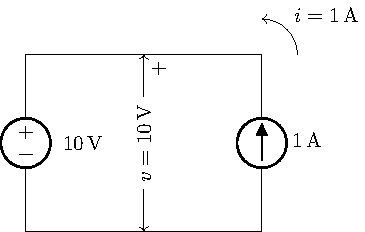
\includegraphics[height = 4cm, keepaspectratio = true]{connected_sources}
    \caption{Example of a connected voltage and current source.}
\end{figure}
\begin{itemize}
    \item The voltage source sets $v$ to \SI{10}{\volt}, with the upper wire being positive.
    \item The current source sets $i$ to \SI{1}{\ampere}, flowing anticlockwise.
    \item Therefore \SI{10}{\watt} of power is produced by the current source and dissipated by the voltage source.
\end{itemize}
\begin{enumerate}
    \item Two voltage sources must be connected at the same terminals and supply the same voltage.
    \item Two current sources must flow in the same direction and supply the same current.
\end{enumerate}
% \subsection{Invalid Circuits}
% \begin{figure}[H]
%     \centering
%     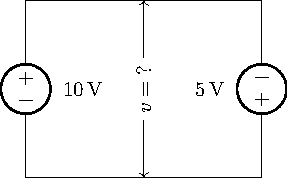
\includegraphics[height = 4cm, keepaspectratio = true]{invalid_voltage_sources}
%     \caption{Voltage terminals are incorrect, and voltages are different.}
% \end{figure}
% \begin{figure}[H]
%     \centering
%     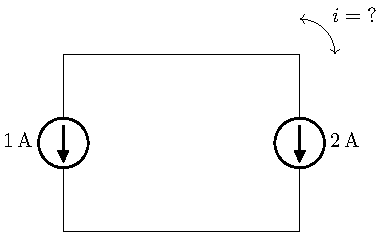
\includegraphics[height = 4cm, keepaspectratio = true]{invalid_current_sources}
%     \caption{Current flows oppose each other, and currents are different.}
% \end{figure}
\subsection{Resistors}
\begin{definition}[Resistor]
    Resistors dissipate power, and the voltage across both terminals is proportional to the current.
\end{definition}
\begin{figure}[H]
    \centering
    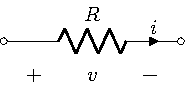
\includegraphics[height = 4cm, keepaspectratio = true]{resistor}
    \caption{Resistor Circuit Symbol}
\end{figure}
\begin{theorem}[Voltage through a resistor]
    \begin{equation*}
        v=iR
    \end{equation*}
    % \begin{equation*}
    %     R=\frac{\rho L}{A}
    % \end{equation*}
\end{theorem}
\begin{corollary}[Power dissipated by a resistor]
    \begin{equation*}
	p = vi = i^2 R = \frac{v^2}{R}
    \end{equation*}
\end{corollary}
\newpage
\section{Simple Resistive Circuits}
\subsection{Ignored Physics}
\begin{enumerate}
    \item Electrical effects occur instantaneously, so there is no time delay along the wires.
    \item The net charge on every component is zero. Charge is never lost or gained.
    \item There is no magnetic coupling between the components.
\end{enumerate}
\subsection{Kirchhoff's Laws}
\begin{definition}[Kirchhoff's Current Law (KCL)]
    The sum of all currents into a node equals zero.
    \begin{equation*}
        \sum i_{\mathrm{node}} = 0
    \end{equation*}
\end{definition}
\begin{definition}[Kirchhoff's Voltage Law (KVL)]
    The sum of all voltages around a loop equals zero.
    \begin{equation*}
        \sum v_{\mathrm{loop}} = 0
    \end{equation*}
\end{definition}
\subsection{Series and Parallel Circuits}
\begin{definition}
    Elements connected end-to-end are in series. If both ends of an element are connected directly to another element, the two elements are in parallel.
\end{definition}
\begin{table}[H]
    \centering
    \begin{tabular}{c | c c}
        \toprule
        \textbf{Element} &  \textbf{Series} & \textbf{Parallel} \\
        \midrule
        Current Source & $\displaystyle i_{eq} = i_{k\geq1}$             & $i_{eq} = \displaystyle \sum_{k\geq1} i_k$ \\
        Voltage Source & $\displaystyle v_{eq} = \sum_{k\geq1} v_k$                     & $\displaystyle v_{eq} = v_{k\geq1}$ \\
        Resistor       & $\displaystyle R_{eq} = \sum_{k\geq1} R_k$                     & $\displaystyle \frac{1}{R_{eq}} = \sum_{k\geq1} \frac{1}{R_k}$ \\
        Inductor       & $\displaystyle L_{eq} = \sum_{k\geq1} L_k$                     & $\displaystyle \frac{1}{L_{eq}} = \sum_{k\geq1} \frac{1}{L_k}$ \\
        Capacitor      & $\displaystyle \frac{1}{C_{eq}} = \sum_{k\geq1} \frac{1}{C_k}$ & $\displaystyle C_{eq} = \sum_{k\geq1} C_k$ \\
        \bottomrule
    \end{tabular}
    \caption{Equivalent values for various components connected in series and parallel.}
    % \label{}
\end{table}
These equations can be used to simplify a complex circuit.
% \begin{proof}
%     Using KVL for voltage sources connected in series
%     \begin{align*}
%         v_1 + v_2 + \cdots + v_n - iR &= 0 \\
%         v_1 + v_2 + \cdots + v_n &= iR
%     \end{align*}
%     Let $v_{eq}$ be the voltage across the resistor so that
%     \begin{equation*}
%         v_{eq} = iR
%     \end{equation*}
%     Therefore
%     \begin{equation*}
%         v_{eq} = v_1 + v_2 + \cdots + v_n
%     \end{equation*}
    
%     As the current through resistors in series remains the same, using KVL we have
%     \begin{align*}
%         v - iR_1 - iR_2 - \cdots - iR_n &= 0 \\
%         v &= i\left(R_1 + R_2 + \cdots + R_n\right) \\
%         v &= iR_{eq}
%     \end{align*}
%     Hence the resistance across multiple resistors in series is equivalent to the sum of the resistances.
% \end{proof}
\subsection{Voltage and Current Dividers}
\begin{definition}[Voltage Divider]
    A voltage divider is a circuit that divides a voltage in the proportion of the series resistances.
\end{definition}
\begin{figure}[H]
    \centering
    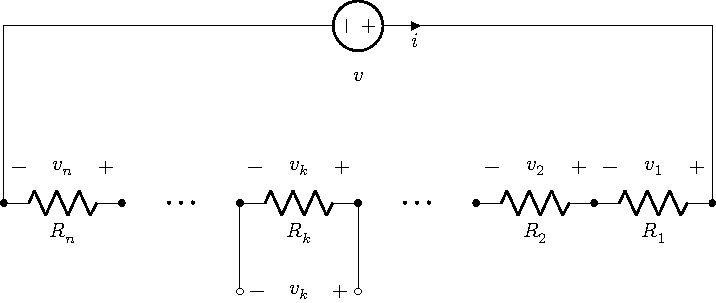
\includegraphics[height = 4cm, keepaspectratio = true]{voltage_divider}
    \caption{Resistors connected in series to a voltage source.}
    % \label{}
\end{figure}
\begin{theorem}
    \begin{equation*}
        v_k = v \frac{R_k}{R_{eq}}
    \end{equation*}
\end{theorem}
\begin{proof}
    The current through any resistor is
    \begin{equation*}
        i = \frac{v}{R_{eq}}
    \end{equation*}
    Therefore the voltage drop in any resistor is
    \begin{align*}
        v_k &= i R_k \\
        v_k &= \frac{v}{R_{eq}} R_k
    \end{align*}
\end{proof}
\begin{definition}[Current Divider]
    A voltage divider is a circuit that divides a voltage in the proportion of the series resistances.
\end{definition}
\begin{figure}[H]
    \centering
    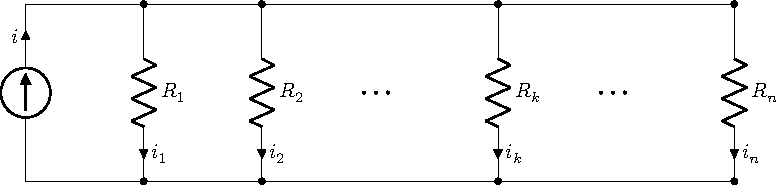
\includegraphics[height = 3cm, keepaspectratio = true]{current_divider}
    \caption{Resistors connected in parallel to a current source.}
    % \label{}
\end{figure}
\begin{theorem}
    \begin{equation*}
        i_k = i \frac{R_{eq}}{R_k}
    \end{equation*}
\end{theorem}
\begin{proof}
    Using KCL we have
    \begin{align*}
        i &= \sum_{k\geq1} i_k \\
        i &= \sum_{k\geq1} \frac{v}{R_k} \\
        i &= \frac{v}{R_{eq}}
    \end{align*}
    Solving for $v$ gives
    \begin{align*}
        v &= i R_{eq} 
    \end{align*}
    Hence the current through any resistor in parallel is given by
    \begin{align*}
        i_k = \frac{v}{R_k} = \frac{iR_{eq}}{R_k}
    \end{align*}
\end{proof}
\newpage 
\section{Diodes}
\begin{definition}[Diode]
    A diode is a semiconductor component in which current flows only in one direction. A diodes requires a voltage to start the flow of current in the forward direction.
\end{definition}
\begin{figure}[H]
    \centering
    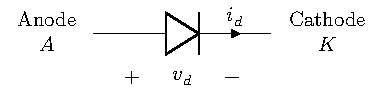
\includegraphics[height = 3cm, keepaspectratio = true]{diode}
    \caption{Diode Circuit Symbol}
    % \label{}
\end{figure}
\subsection{V-I Characteristic}
The Voltage-Current characteristic of linear circuit elements can be plotted as shown below.
\begin{figure}[H]
    \centering
    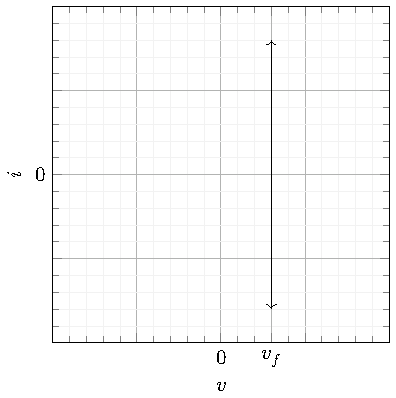
\includegraphics[height = 5cm, keepaspectratio = true]{vi_characteristic_voltage_source}
    \caption{V-I characteristic for a voltage source.}
    % \label{}
\end{figure}
\begin{figure}[H]
    \centering
    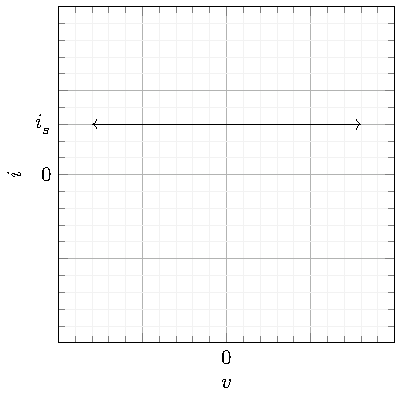
\includegraphics[height = 5cm, keepaspectratio = true]{vi_characteristic_current_source}
    \caption{V-I characteristic for a current source.}
    % \label{}
\end{figure}
\begin{figure}[H]
    \centering
    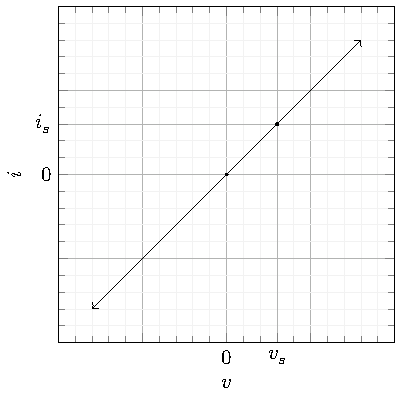
\includegraphics[height = 5cm, keepaspectratio = true]{vi_characteristic_resistor}
    \caption{V-I characteristic for a resistor.}
    % \label{}
\end{figure}
\subsection{V-I Characteristic for Diodes}
A diode has a non-linear characteristic curve, hence it is often simplified.
\begin{figure}[H]
    \centering
    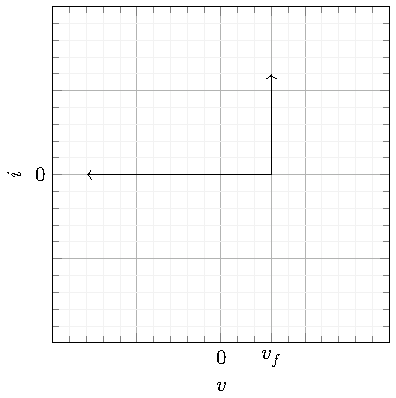
\includegraphics[height = 5cm, keepaspectratio = true]{vi_characteristic_diode}
    \caption{V-I characteristic for a diode.}
    % \label{}
\end{figure}
\begin{theorem}[Shockley's Diode Equation]
    A diode can be better modelled using Shockley's equation.
    \begin{equation*}
        i_D = I_S \exp{\left( \frac{v_D}{0.026} \right)}
    \end{equation*}
    where $I_S$ is the saturation current and $0.026$ is the thermal voltage. 
\end{theorem}
\subsection{Operating Points and Load Lines}
\begin{definition}[Operating Point]
    The operating point for two elements can be found by determining the intersection 
    of the two V-I characteristic curves.
\end{definition}
\begin{definition}[Load Lines]
    If a circuit contains three or more elements including a diode, the V-I characteristic curve
    is found around the diode. This curve is called a load line.
\end{definition}
\subsection{Operating Point of Non-Linear Component}
Given the following circuit with a non-linear component
\begin{figure}[H]
    \centering
    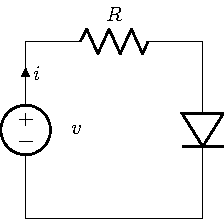
\includegraphics[height = 4cm, keepaspectratio = true]{non_linear_component}
    \caption{Circuit with non-linear element.}
    % \label{}
\end{figure}
the load line is given by the equation
\begin{equation*}
    i(v) = -\frac{i_{sc}}{v_{oc}} + i_{sc}
\end{equation*}
where the short-circuit current is the current through the non-linear component, and the open circuit voltage is the voltage across the 
open circuit nodes of the component.
\begin{figure}[H]
    \centering
    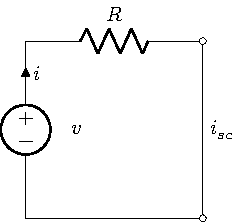
\includegraphics[height = 4cm, keepaspectratio = true]{non_linear_short_circuit_current}
    \caption{Circuit for Short Circuit Current.}
    % \label{}
\end{figure}
\begin{figure}[H]
    \centering
    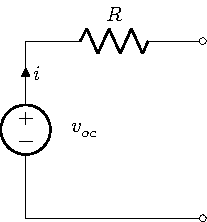
\includegraphics[height = 4cm, keepaspectratio = true]{non_linear_open_circuit_voltage}
    \caption{Circuit for Open Circuit Voltage.}
    % \label{}
\end{figure}
\newpage
\section{Mesh Analysis}
\begin{definition}[Node]
    A point where two or more circuit elements join.
\end{definition}
\begin{definition}[Essential Node]
    A point where three or more circuit elements join.
\end{definition}
\begin{definition}[Loop]
    A path with the same start and end node.
\end{definition}
\begin{definition}[Mesh]
    A loop that does not enclose any other loops.
\end{definition}
\subsection{Mesh Analysis Steps}
\begin{enumerate}
    \item Label the unknown mesh currents.
    \item Find the voltage across each of the circuit elements in terms of mesh currents.
    \item Use KVL around each mesh to create simultaneous equations.
    \item Solve simultaneous equations for mesh currents.
\end{enumerate}
\subsection{Mesh Analysis with Current Sources}
If the current source is in a single mesh, then treat the mesh current as known and solve as before.

If the current source is between two meshes, then we must use a supermesh.
\begin{definition}[Supermesh]
    A supermesh is a special mesh that surrounds the current source.
\end{definition}
\begin{enumerate}
    \item Label meshes and identify supermesh.
    \item Write KCL equation for current source.
    \item Write supermesh equation.
    \item Use KVL around supermesh.
\end{enumerate}
\newpage
\section{Source Transformations}
Real sources often have many limitations in terms of voltage and current delivery.
The most commonly modelled, and most useful for linear circuit theory, is some form of 
resistance associated with the source.
\subsection{Thévenin Equivalent Circuit}
\begin{definition}
    The Thévenin equivalent circuit is a voltage source with a series resistance.
    \begin{figure}[H]
        \centering
        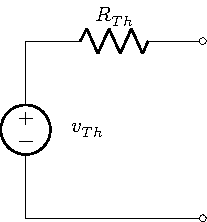
\includegraphics[height = 4cm, keepaspectratio = true]{thevenin_equivalent}
        \caption{Thévenin Equivalent Circuit.}
        % \label{}
    \end{figure}
    This circuit has the following properties:
    \begin{description}
        \item[Open circuit voltage.] $v_{oc} = v_{Th}$
        \item[Short circuit current.] $i_{sc} = \frac{v_{Th}}{R_{Th}}$
    \end{description}
\end{definition}
\subsection{Norton Equivalent Circuit}
\begin{definition}
    Similar to the Thévenin equivalent model, we can use a current source with 
    a resistor in parallel to model the same circuit.
    \begin{figure}[H]
        \centering
        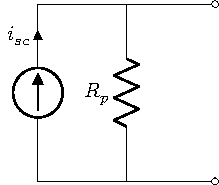
\includegraphics[height = 4cm, keepaspectratio = true]{norton_equivalent}
        \caption{Norton Equivalent Circuit.}
        % \label{}
    \end{figure}
    This circuit has the following properties:
    \begin{description}
        \item[Open circuit voltage.] $v_{oc} = i_{sc}R_{p}$
        \item[Short circuit current.] $i_{sc} = i_{sc}$ 
    \end{description}
\end{definition}
\subsection{Source Transformations}
A source transformation is the process of simplifying a circuit by transforming 
voltage sources into current sources, and vice versa, using Thévenin's Theorem and Norton's 
Theorem.
\begin{theorem}
    Thévenin and Norton equivalent circuits have the following relationship
    \begin{equation*}
        R_{Th} = R_{p}
    \end{equation*}
\end{theorem}
\subsection{Superposition}
\begin{theorem}[Thévenin's Theorem]
    Any linear circuit can be replaced by a voltage source and a resistance in series.
\end{theorem}
\begin{theorem}[Norton's Theorem]
    Any linear circuit can be replaced by a current source and a resistance in parallel.
\end{theorem}
\subsection{Maximum Power Transfer}
In the circuit shown below, the maximum power transfer to the load is given by
\begin{equation*}
    P_L = \frac{v_{Th}^2}{4R_L}.
\end{equation*}
\begin{figure}[H]
    \centering
    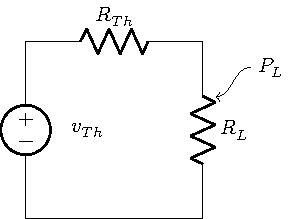
\includegraphics[height = 4cm, keepaspectratio = true]{max_power_transfer}
    \caption{Power Transfer in a Thévenin Model.}
    % \label{}
\end{figure}
\newpage
\section{Inductors and Capacitors}
\subsection{Capacitors}
\begin{definition}
    Capacitors store electrical energy as a voltage. The ratio of voltage 
    to charge across a capacitor is its capacitance, measured in Farads (\si{\farad}).
    \begin{equation*}
        q = C v
    \end{equation*}
\end{definition}
\begin{definition}[VI Relationship]
    \begin{equation*}
        i = C \dv{v}{t}
    \end{equation*}
    \begin{equation*}
        v(t) = \frac{1}{C} \int_0^t i(\tau) \dd{\tau} + v(0)
    \end{equation*}
\end{definition}
\begin{definition}[Energy Stored by an Capacitor]
    \begin{equation*}
        W = \frac{1}{2}Cv^2
    \end{equation*}
\end{definition}
\begin{theorem}[Steady State Conditions]
    When a circuit is in steady state, capacitors can be modelled as open circuits.
\end{theorem}
\subsection{Inductors}
\begin{definition}
    Inductors create voltage to oppose a change in current. The ratio of voltage 
    to the rate of change of current through an inductor is its inductance, measured in Henrys (\si{\henry}).
\end{definition}
\begin{definition}[VI Relationship]
    \begin{equation*}
        v = L \dv{i}{t}
    \end{equation*}
    \begin{equation*}
        i(t) = \frac{1}{L} \int_0^t v(\tau) \dd{\tau} + i(0)
    \end{equation*}
\end{definition}
\begin{definition}[Energy Stored by an Inductor]
    \begin{equation*}
        W = \frac{1}{2}Li^2
    \end{equation*}
\end{definition}
\begin{theorem}[Steady State Conditions]
    When a circuit is in steady state, inductors can be modelled as short circuits.
\end{theorem}
\newpage
\section{RC and RL Circuits}
\subsection{Switches}
\begin{definition}
    A switch will engage part of a circuit at a specified point in time, as indicated 
    on the circuit diagram.
\end{definition}
\begin{definition}[Poles]
    ``Pole'' refers to the number of circuits one switch can control.
\end{definition}
\begin{definition}[Throw]
    ``Throw'' refers to the number of output connections each switch 
    pole can connect its input to.
\end{definition}
\subsection{Natural Response}
\begin{definition}[RC Circuit Natural Response]
    For the circuit shown below, using KCL gives the following relationship
    \begin{equation*}
        -C \dv{v}{t} = \frac{v}{R}.
    \end{equation*}
    \begin{figure}[H]
        \centering
        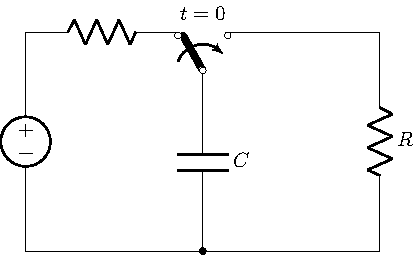
\includegraphics[height = 4cm, keepaspectratio = true]{rc_natural}
        \caption{RC Circuit.}
        % \label{}
    \end{figure}
    By solving this differential equation, we can determine the natural response of a 
    RC circuit.
    \begin{equation*}
        v(t) = v(0)\exp{\left( -\frac{t}{RC} \right)}
    \end{equation*}
    \begin{figure}[H]
        \centering
        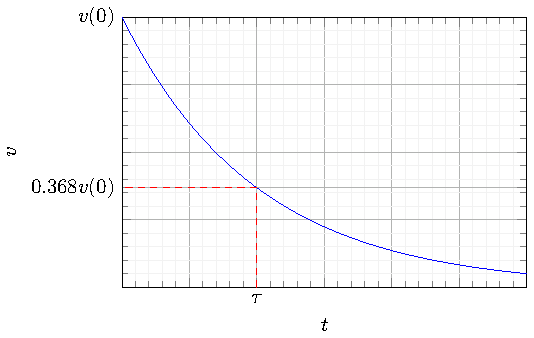
\includegraphics[height = 4cm, keepaspectratio = true]{rc_natural_plot}
        \caption{Natural Response of a RC Circuit.}
        % \label{}
    \end{figure}
\end{definition}
\begin{definition}[Time Constant]
    The time constant $\tau$ is a parameter for switching circuits. The time constant for a RC circuit is given by
    \begin{equation*}
        \tau = RC
    \end{equation*}
    The voltage at this time is equal to
    \begin{equation*}
        \e^{-1}v(0) \approx 0.368v(0)
    \end{equation*} 
\end{definition}
\begin{definition}[RL Circuit Natural Response]
    For the circuit shown below, using mesh analysis gives the following relationship
    \begin{equation*}
        L \dv{i}{t} = -iR.
    \end{equation*}
    \begin{figure}[H]
        \centering
        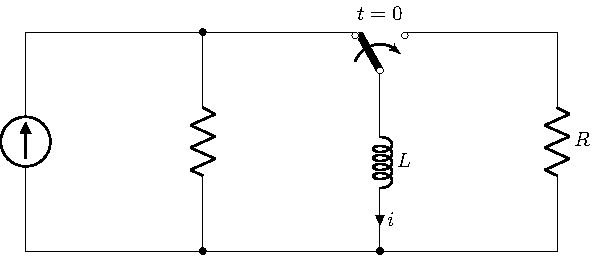
\includegraphics[height = 4cm, keepaspectratio = true]{rl_natural}
        \caption{RL Circuit.}
        % \label{}
    \end{figure}
    By solving this differential equation, we can determine the natural response of a 
    RL circuit.
    \begin{equation*}
        i(t) = i(0)\exp{\left( -\frac{t}{\frac{1}{R}L} \right)}
    \end{equation*} 
    \begin{figure}[H]
        \centering
        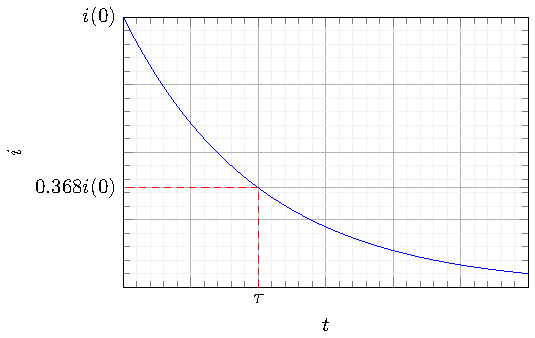
\includegraphics[height = 4cm, keepaspectratio = true]{rl_natural_plot}
        \caption{Natural Response of a RL Circuit.}
        % \label{}
    \end{figure}
\end{definition}
\begin{definition}[Time Constant]
    The time constant $\tau$ is a parameter for switching circuits. The time constant for a RL circuit is given by
    \begin{equation*}
        \tau = \frac{1}{R}L
    \end{equation*}
    The current at this time is equal to
    \begin{equation*}
        \e^{-1}i(0) \approx 0.368i(0)
    \end{equation*} 
\end{definition}
\subsection{Step Response}
\begin{definition}[RC Circuit Step Response]
    For the circuit shown below, using KCL at the top node gives the following relationship
    \begin{equation*}
        i_s = C\dv{v}{t} + \frac{v}{R}.
    \end{equation*}
    \begin{figure}[H]
        \centering
        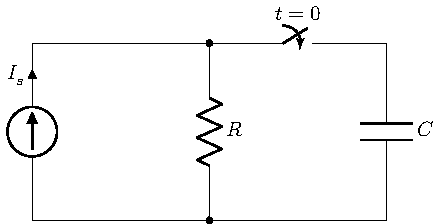
\includegraphics[height = 4cm, keepaspectratio = true]{rc_step}
        \caption{RC Circuit.}
        % \label{}
    \end{figure}
    By solving this differential equation, we can determine the step response of a 
    RC circuit.
    \begin{equation*}
        v(t) = I_sR + \left(V_0 - I_sR\right) \exp{\left( -\frac{t}{RC} \right)}
    \end{equation*}
    \begin{figure}[H]
        \centering
        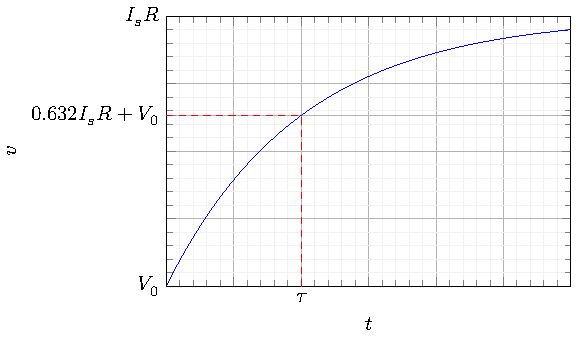
\includegraphics[height = 4cm, keepaspectratio = true]{rc_step_plot}
        \caption{Step Response of a RC Circuit.}
        % \label{}
    \end{figure}
    The voltage at $t=\tau$ is equal to
    \begin{align*}
        v(\tau) &= \left(1 - \e^{-1}\right)I_sR + V_0 \\
        &\approx 0.632I_sR + V_0
    \end{align*} 
\end{definition}
\begin{definition}[RL Circuit Step Response]
    For the circuit shown below, using mesh analysis gives the following relationship
    \begin{equation*}
        L\dv{i}{t} + iR = V_s.
    \end{equation*}
    \begin{figure}[H]
        \centering
        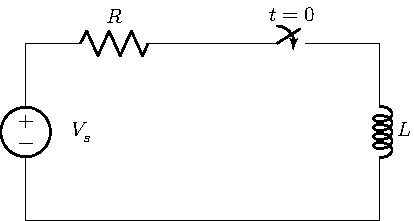
\includegraphics[height = 4cm, keepaspectratio = true]{rl_step}
        \caption{RL Circuit.}
        % \label{}
    \end{figure}
    By solving this differential equation, we can determine the step response of a 
    RL circuit.
    \begin{equation*}
        i(t) = \frac{V_s}{R} + \left(I_0 - \frac{V_s}{R}\right)\exp{\left( -\frac{t}{\frac{1}{R}L} \right)}
    \end{equation*} 
    \begin{figure}[H]
        \centering
        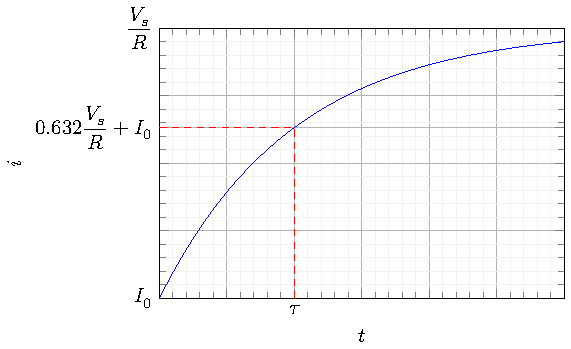
\includegraphics[height = 4cm, keepaspectratio = true]{rl_step_plot}
        \caption{Step Response of a RL Circuit.}
        % \label{}
    \end{figure}
    The current at $t=\tau$ is equal to
    \begin{align*}
        i(\tau) &= \left( 1 - \e^{-1} \right)\frac{V_s}{R} + I_0 \\
        &\approx 0.632\frac{V_s}{R} + I_0
    \end{align*} 
\end{definition}
\newpage
\section{Operational Amplifiers}
\begin{definition}[Amplifier]
    An amplifier is a device for increasing the power of a signal through an external energy source. 
    In an electronic amplifier, the ``signal'' is usually a voltage or current.
\end{definition}
\begin{definition}[Gain]
    The gain $K$ of an amplifier, is the ratio of the output signal to the input signal.
    \begin{equation*}
        v_{out} = K v_{in}
    \end{equation*}
\end{definition}
\begin{definition}[Operational Amplifier]
    An operational amplifier amplifies the voltage difference between its input terminals. 
    Operational amplifiers require a power supply to amplify voltage.
    In an operational amplifier:
    \begin{enumerate}
        \item The output cannot exceed the power supply range.
        \item The inputs should remain within the power supply range.
    \end{enumerate}
    The output voltage has the following possibilities:
    \begin{enumerate}
        \item If $v_p - v_n > 0$, $v_{out} = V_{CC}$. 
        \item If $v_p - v_n < 0$, $v_{out} = V_{EE}$. 
        \item If $v_p - v_n = 0$, $v_{out} = 0$. 
    \end{enumerate}
    where $v_p$ is the non-inverting input, $v_n$ is the inverting input, $V_{CC}$ is the positive power supply voltage and 
    $V_{EE}$ is the negative power supply voltage.
    \begin{figure}[H]
        \centering
        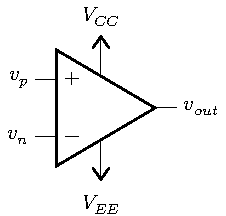
\includegraphics[height = 4cm, keepaspectratio = true]{operational_amplifier}
        \caption{Operational Amplifier Circuit Symbol.}
        % \label{}
    \end{figure}
\end{definition}
\newpage
\section{Sinusoidal Signals}
\newpage
\section{Frequency Response}
\newpage
\section{Filters and Rectifiers}
\newpage
\section{Zener Diodes and Voltage Regulators}
\newpage

\end{document}